\de{ĐỀ THI HỌC KỲ II NĂM HỌC 2022-2023}{Phổ Thông Năng Khiếu}


% câu 1
\begin{bt}%[0T7K2-2]%[Dự án đề kiểm tra HKII NH22-23- Hiếu Mai]%[Phổ thông năng khiếu]
Giải bất phương trình $ \dfrac{-3+4x-x^{2}}{x^{2}-5x+6} \le 0 $.
\loigiai{
Ta có
$$
	\dfrac{-3+4x-x^{2}}{x^{2}-5x+6} \le 0
	\Leftrightarrow
	\dfrac{x^{2}-4x+3}{x^{2}-5x+6} \ge 0 \quad (1)
$$
Dựa vào bảng xét dấu
\begin{center} 
\begin{tikzpicture} 
	\tkzTabInit[lgt=3,espcl=2] {$x$ /1, $x^2-4x+3$ /1, $ x^{2}-5x+6 $/1, $ VT(1) $/1} {$ -\infty $, $ 1 $, $ 2 $, $ 3 $, $ +\infty $} 
	\tkzTabLine{ , +, z, -, t, -, z, + } 
	\tkzTabLine{ , +, t, +, z, -, z, + } 
	\tkzTabLine{ , +, z, -, d, +, d, + } 
\end{tikzpicture}
\end{center}
ta thấy bất phương trình đã cho có tập nghiệm
$ S = \left(-\infty;1 \right] \cup \left( 2;3 \right) \cup \left( 3;+\infty \right) $.
}
\end{bt}

% câu 2
\begin{bt}%[0T7G2-2]%[Dự án đề kiểm tra HKII NH22-23- Hiếu Mai]%[Phổ thông năng khiếu]
Tìm $ m $ để hàm số
$$
	y = \sqrt{
		\dfrac{-2x^{2}-10}
		{mx^{2}+2mx-2}
	}
$$
xác định với mọi $ x \in \mathbb{R} $.
\loigiai{
Đặt $ f(x) = \dfrac{-2x^{2}-10}
		{mx^{2}+2mx-2} $ thì yêu cầu bài toán tương đương với
$$
	f(x) \ge 0, \, \forall x \in \mathbb{R}
$$
Mà $ -2x^{2}-10 \le -10 < 0, \, \forall x \in \mathbb{R} $ nên
$$
	mx^{2}+2mx-2 < 0, \, \forall x \in \mathbb{R} \quad (1)
$$
\begin{itemize}
	\item Nếu $ m = 0 $ thì
	$$
		(1)
		\Leftrightarrow
		-2 < 0, \, \forall x \in \mathbb{R} \quad 			\text{(luôn đúng)}
	$$
	
	\item Nếu $ m \ne 0 $ thì
	$$
		(1)
		\Leftrightarrow
		\heva{
			&m < 0
			\\
			&\Delta = (2m)^{2}-4(m)(-2) < 0
		}
		\Leftrightarrow
		\heva{
			&m < 0
			\\
			&4m^{2}+8m < 0
		}
		\Leftrightarrow
		\heva{
			&m < 0
			\\
			&m+2 > 0
		}
		\Leftrightarrow
		-2<m<0
	$$
\end{itemize}
Vậy $ -2 < m \le 0 $ thỏa mãn yêu cầu bài toán.

}
\end{bt}

% câu 3
\begin{bt}%[0T8G1-2]%[Dự án đề kiểm tra HKII NH22-23- Hiếu Mai]%[Phổ thông năng khiếu]
\begin{enumerate}
	\item Tìm số hạng không chứa $ x $ trong khai triển
	$$ x^{2} \left( \dfrac{2}{x^{3}}-x^{2} \right)^{4} $$
	\item Một lớp có $ 15 $ học sinh nam và $ 10 $ học sinh nữ. Có bao nhiêu cách chọn ra một đội văn nghệ gồm $ 6 $ học sinh có cả nam lẫn nữ.
	\item Cho $ X = \{ 0,\,1,\,2,\,3,\,4,\,5,\,6,\,7,\,8 \} $. Chọn ngẫu nhiên một số có $ 4 $ chữ số được lập từ $ X $. Tính xác suất số được chọn là số chẵn và có các chữ số phân biệt.
\end{enumerate}
\loigiai{
\begin{enumerate}
	\item Tìm số hạng không chứa $ x $ trong khai triển
	$$ x^{2} \left( \dfrac{2}{x^{3}}-x^{2} \right)^{4} $$
	Khai triển biểu thức trên, ta được
	\begin{align*}
		x^{2} \left( \dfrac{2}{x^{3}}-x^{2} \right)^{4}
		&= x^{2} \left[
			C_{4}^{0}\left( \dfrac{2}{x^{3}} \right)^{4}\left( x^{2} \right)^{0} - 
			C_{4}^{1}\left( \dfrac{2}{x^{3}} \right)^{3}\left( x^{2} \right)^{1} 
			\right. \\
			&\qquad\qquad \left.+ C_{4}^{2}\left( \dfrac{2}{x^{3}} \right)^{2}\left( x^{2} \right)^{2} - 
			C_{4}^{3}\left( \dfrac{2}{x^{3}} \right)^{1}\left( x^{2} \right)^{3} + 
			C_{4}^{4}\left( \dfrac{2}{x^{3}} \right)^{0}\left( x^{2} \right)^{4} 
		\right]
		\\
		&= x^{2} \left(
			\dfrac{16}{x^{12}} - \dfrac{32}{x^{7}}  + \dfrac{24}{x^{2}} - 8x^{3} + x^{8}
		\right)
		\\
		&= \dfrac{16}{x^{10}} - \dfrac{32}{x^{5}}  + 24 - 8x^{5} + x^{10}
	\end{align*}
	Như vậy số hạng không chứa $ x $ là $ 24 $.
	
	\item Một lớp có $ 15 $ học sinh nam và $ 10 $ học sinh nữ. Có bao nhiêu cách chọn ra một đội văn nghệ gồm $ 6 $ học sinh có cả nam lẫn nữ.
	\\
	Số cách chọn ra $ 6 $ bạn cách tùy ý là 
	$$ \mathrm{C}_{25}^{6} = 177\,100 $$
	Số cách chọn ra 6 bạn chỉ có nam hoặc chỉ có nữ là 
	$$ \mathrm{C}_{15}^{6} + \mathrm{C}_{10}^{6} = 5\,215  $$
	Số cách chọn ra 6 bạn có đủ cả nam lẫn nữ là 
	$$ 177\,100 - 5\,215 = 171\,885 $$
	
	\item Cho $ X = \{ 0,\,1,\,2,\,3,\,4,\,5,\,6,\,7,\,8 \} $. Chọn ngẫu nhiên một số có $ 4 $ chữ số được lập từ $ X $. Tính xác suất số được chọn là số chẵn và có các chữ số phân biệt.
	\\
	Gọi $ A $ là biến cố: \lq\lq Số được chọn là số chẵn và có các chữ số phân biệt.\rq\rq
	\\
	Gọi  số có $ 4 $ chữ số đôi một khác nhau $ \overline{abcd} $ được lập từ $ X $ thì
	\begin{itemize}
		\item Chọn $ a $ từ $ X\backslash \{ 0 \} $ có $ 8 $ cách
		\item Chọn $ b,c,d $ từ $ X \backslash \{ a \} $ có $ \mathrm{A}_{8}^{3} = 336 $ cách.
	\end{itemize}
	Theo quy tắc nhân ta lập được $ 8 \cdot 336 = 2\,688 $ cách. Do đó số phần từ của không gian mẫu là 
	$$
		n(\Omega) = 2\,688
	$$
	\\
	Để lập được số chẵn thì
	\\
	\textbf{Trường hợp 1:} $ d = 0 $
	\begin{itemize}
		\item Chọn $ d $ có $ 1 $ cách.
		\item Chọn $ a,b,c $ từ $ X \backslash \{ d \} $ có $ \mathrm{A}_{8}^{3} $ cách.
	\end{itemize}
	
	\textbf{Trường hợp 2:} $ d \ne 0 $
	\begin{itemize}
		\item Chọn $ d $ từ $ \{ 2,\,4,\,6,\,8 \} $ có $ 4 $ cách.
		\item Chọn $ a $ từ $ X \backslash \{ 0,\,d \} $ có $ 7 $ cách.
		\item Chọn $ b,c $ từ $ X \backslash \{ a,\,d \} $ có $ \mathrm{A}_{7}^{2} $ cách.
	\end{itemize}
	Theo quy tắc cộng và nhân, ta lập được $ 1 \cdot \mathrm{A}_{8}^{3} + 4 \cdot 7 \cdot \mathrm{A}_{7}^{2} = 1\,512 $ cách. 
	\\
	Do đó số phần tử của $ A $ là
	$$
		n(A) = 1\,512
	$$
	Vậy xác suất của biến cố $ A $
	$$
		P(A) = \dfrac{n(A)}{n(\Omega)}
		= \dfrac{1\,512}{2\,688} = \dfrac{9}{16}
	$$
\end{enumerate}
}
\end{bt}

\begin{bt}%[Dự án đề kiểm tra HKII NH22-23- Mui Doan]%[0T9B2-2]%[0T9B3-2]%[0T9K1-3]
Cho hai điểm $A(1;2)$, $B(3;6)$ và đường thẳng $(\Delta)\colon x+y-3=0$.
	\begin{enumerate}
		\item Viết phương trình đường thẳng $AB$.
		\item Viết phương trình đường tròn có tâm $B$ và tiếp xúc với đường thẳng $(\Delta)$.
		\item Tìm trên $(\Delta)$ điểm $M$ sao cho $AM=\sqrt{2}$.
	\end{enumerate}
\loigiai{
\begin{enumerate}
	\item Viết phương trình đường thẳng $AB$.\\
	Ta có $\overrightarrow{AB}=(2;4)=2(1;2)$.\\
	$AB$ qua $A$ và có một véc-tơ chỉ phương là $\overrightarrow{u}=(1;2)\Rightarrow \overrightarrow{n}=(2;-1)$ là một véc-tơ pháp tuyến, do đó $AB$ có phương trình là $2(x-1)-1(y-2)=0\Leftrightarrow 2x-y=0$.
	\item Viết phương trình đường tròn có tâm $B$ và tiếp xúc với đường thẳng $(\Delta)$.\\
	Gọi $(C)$ là đường tròn tâm $B$ và tiếp xúc với đường thẳng $(\Delta)$.\\
	Ta có bán kính $R=\mathrm{d}\left(B,(\Delta)\right)=\dfrac{\vert 3+6-3\vert}{\sqrt{1^2+1^2}}=3\sqrt{2}$.\\
	Vậy $(C)\colon (x-3)^2+(y-6)^2= 18$.
	\item Tìm trên $(\Delta)$ điểm $M$ sao cho $AM=\sqrt{2}$.\\
	Vì $M\in(\Delta)\Rightarrow M(m;3-m)$.\\
	Ta có 
	\allowdisplaybreaks
	\begin{eqnarray*}
		&&AM=\sqrt{2}\Leftrightarrow (m-1)^2+(3-m-2)^2=2
		\\
		&\Leftrightarrow& 2(m-1)^2=2\Leftrightarrow (m-1)^2=1
		\\
		&\Leftrightarrow&\hoac{&m-1=1\\&m-1=-1}\Leftrightarrow\hoac{&m=2\\&m=0.}
	\end{eqnarray*}
\end{enumerate}
}
\end{bt}
%Bài 5
\begin{bt}%[Dự án đề kiểm tra HKII NH22-23- Mui Doan]%[PTNK]%[0T9B4-2]
	Lập phương trình chính tắc của elip $(E)$, biết rằng $(E)$ có độ dài trục lớn bằng $8$ và độ dài trục nhỏ bằng $6$.
	\loigiai{
	Ta có $(E)\colon \dfrac{x^2}{a^2}+\dfrac{y^2}{b^2}=1$.\\
	Theo đề bai, ta có $\heva{&2a=8\\&2b=6}\Rightarrow\heva{&a=4\\&b=3.}$	\\
	Vậy $(E)\colon \dfrac{x^2}{16}+\dfrac{y^2}{9}=1$.
	}
\end{bt}

